\documentclass[letterpaper, 10 pt, conference]{article} 
\usepackage[english]{babel}
%\overrideIEEEmargins
% See the \addtolength command later in the file to balance the column lengths
% on the last page of the document
\usepackage{amsmath,amssymb,amscd,amsthm} % variety of useful math macros
\usepackage[inner=1.5 cm, outer = 1.5 cm, top=1 cm, bottom = 1.5 cm]{geometry}
\usepackage{subcaption}
%Para insertar imágenes
\usepackage{graphicx}
\usepackage[dvipsnames]{xcolor}
\usepackage{listings}
\usepackage[utf8]{inputenc}
\usepackage{hyperref}
%Para crear diagramas
%\usepackage{tikz} 



\title{Impact of COVID-19 pandemic in rapid transit ridership in Monterrey, Mexico. }
\author{G. Palafox}

\lstset{ 
	basicstyle=\footnotesize,        % the size of the fonts that are used for the code
	breakatwhitespace=false,         % sets if automatic breaks should only happen at whitespace
	breaklines=true,                 % sets automatic line breaking
	showspaces=false,                % show spaces everywhere adding particular underscores; it overrides 
	showstringspaces = false,
	stringstyle=\color{MidnightBlue},     % string literal style
	backgroundcolor=\color{White},   
}

\begin{document}
\vspace{-2 cm}

\maketitle

\begin{abstract}
In the following report, we make a comparison of passengers transported by Monterrey's rapid transit system (Metrorrey) between the years 2018 and 2020. We show the decrease of ridership expected from the movement restrictions imposed as a response to the current coronavirus pandemic.
\end{abstract}

\section*{Introduction}
The metropolitan area of Monterrey is the third-largest in the country \cite{zonasmetropolitanas}. It is located in north eastern Mexico, south from Texas. Means of transportation in the city include a system of public buses, a rapid transit system, taxis, ride-sharing apps and personal vehicles. The rapid transit system, named Metrorrey, consists of two lines: line one is elevated and line two has an elevated and a subway component \cite{metro}. Metrorrey transported an average of 15.3 million passengers per month in the past two years. As many places around the world, Monterrey has imposed restrictions in the movement of their residents to stop the spread of the coronavirus epidemic. In the next section, we show a brief  analysis of Metrorrey's ridership data, and use our results to observe how impactful the movement restrictions have been on rapid transit ridership.

\section*{Data Analysis}
We obtained Metrorrey's ridership data corresponding to the January 2018 - June 2020 period from \cite{inegi}. To perform a month-to-month comparison between different years, we only considered data from the first six months of each year. That is, we restricted ourselves to the  January-June period for 2018, 2019, and 2020 (see table \ref{tab:1}). Data analysis was performed with R Version 4.0.0 \cite{R} on a Jupyterlab Notebook \cite{jupyter}. 

We processed the data found at \cite{inegi} directly in R \cite{R}. In order to extract information about the months we were interested in, and to create table \ref{tab:1}, we used the following script\footnote{The script and a Jupyter \cite{jupyter} notebook showing how we performed the data analysis and created the graphics in this report can be found at \url{https://github.com/palafox794/AppliedProbabilityModels/tree/master/Assignment1}}:

 \begin{lstlisting}[language=R]
 df <- read.csv(file = 'Tabulado-metrorrey.csv')
 passng = df$Pasajeros.transportados.....Miles.de.pasajeros.
 passng = passng[!is.na(passng)]
 passng2018 = passng[1:6]
 passng2019 = passng[13:18]
 passng2020 = passng[25:30]
 table <- data.frame(c("jan", "feb", "mar", "apr", "may", "jun"), passng2018, passng2019,
  passng2020)
 names(table) <- c("month", "2018", "2019", "2020")
 library("xtable")
 xtable(table)
 \end{lstlisting}
 
 \begin{table}[h!]
 	\centering
 	\begin{tabular}{rlrrr}
 		\hline
 		& Month & 2018 & 2019 & 2020 \\ 
 		\hline
 		1 & jan & 13529.98 & 14534.62 & 15220.38 \\ 
 		2 & feb & 14404.83 & 14511.12 & 15548.33 \\ 
 		3 & mar & 15102.95 & 14659.78 & 12554.89 \\ 
 		4 & apr & 14991.67 & 14826.92 & 5653.46 \\ 
 		5 & may & 15999.97 & 16515.39 & 4933.48 \\ 
 		6 & jun & 14314.63 & 14750.24 & 7208.06 \\ 
 		\hline
 	\end{tabular}
 	\caption{Ridership data (in thousands) to be analysed}
 	\label{tab:1}
 \end{table}

\newpage 
A summary of the data is shown in table \ref{tab:2}, where it can be seen that the smallest values (the minimum, and the first quartile) for ridership in 2020 differ drastically from those of previous years. This can be further shown with the boxplots in figure \ref{fig:boxplots}, the violin plots\footnote{To read more about violin plots, see \cite{violinplot}.} in figure \ref{fig:violinplots} and the bar plot in figure \ref{fig:barplot2018_to_2020}. 

\begin{table}[h!]
	\centering
	\begin{tabular}{rlrrrrrr}
		\hline
		& Year (first half) & Min & 1st Qu. & Median & Mean & 3rd Qu. & Max.  \\ 
		\hline
		1 & 2018 & 13530 & 14337 & 14698 & 14724 & 15075 & 16000 \\ 
		2 & 2019 & 14511 & 14566 & 14705 & 14966 & 14808 & 16515\\ 
		3 & 2020 & 4933 & 6042 & 9881  & 10186 & 14554 & 15548 \\ 
		\hline
	\end{tabular}
	\caption{Ridership data summary. Passengers in thousands.}
	\label{tab:2}
\end{table}

\begin{figure}[h!]
	\centering
	\begin{subfigure}[b]{0.3\linewidth}
		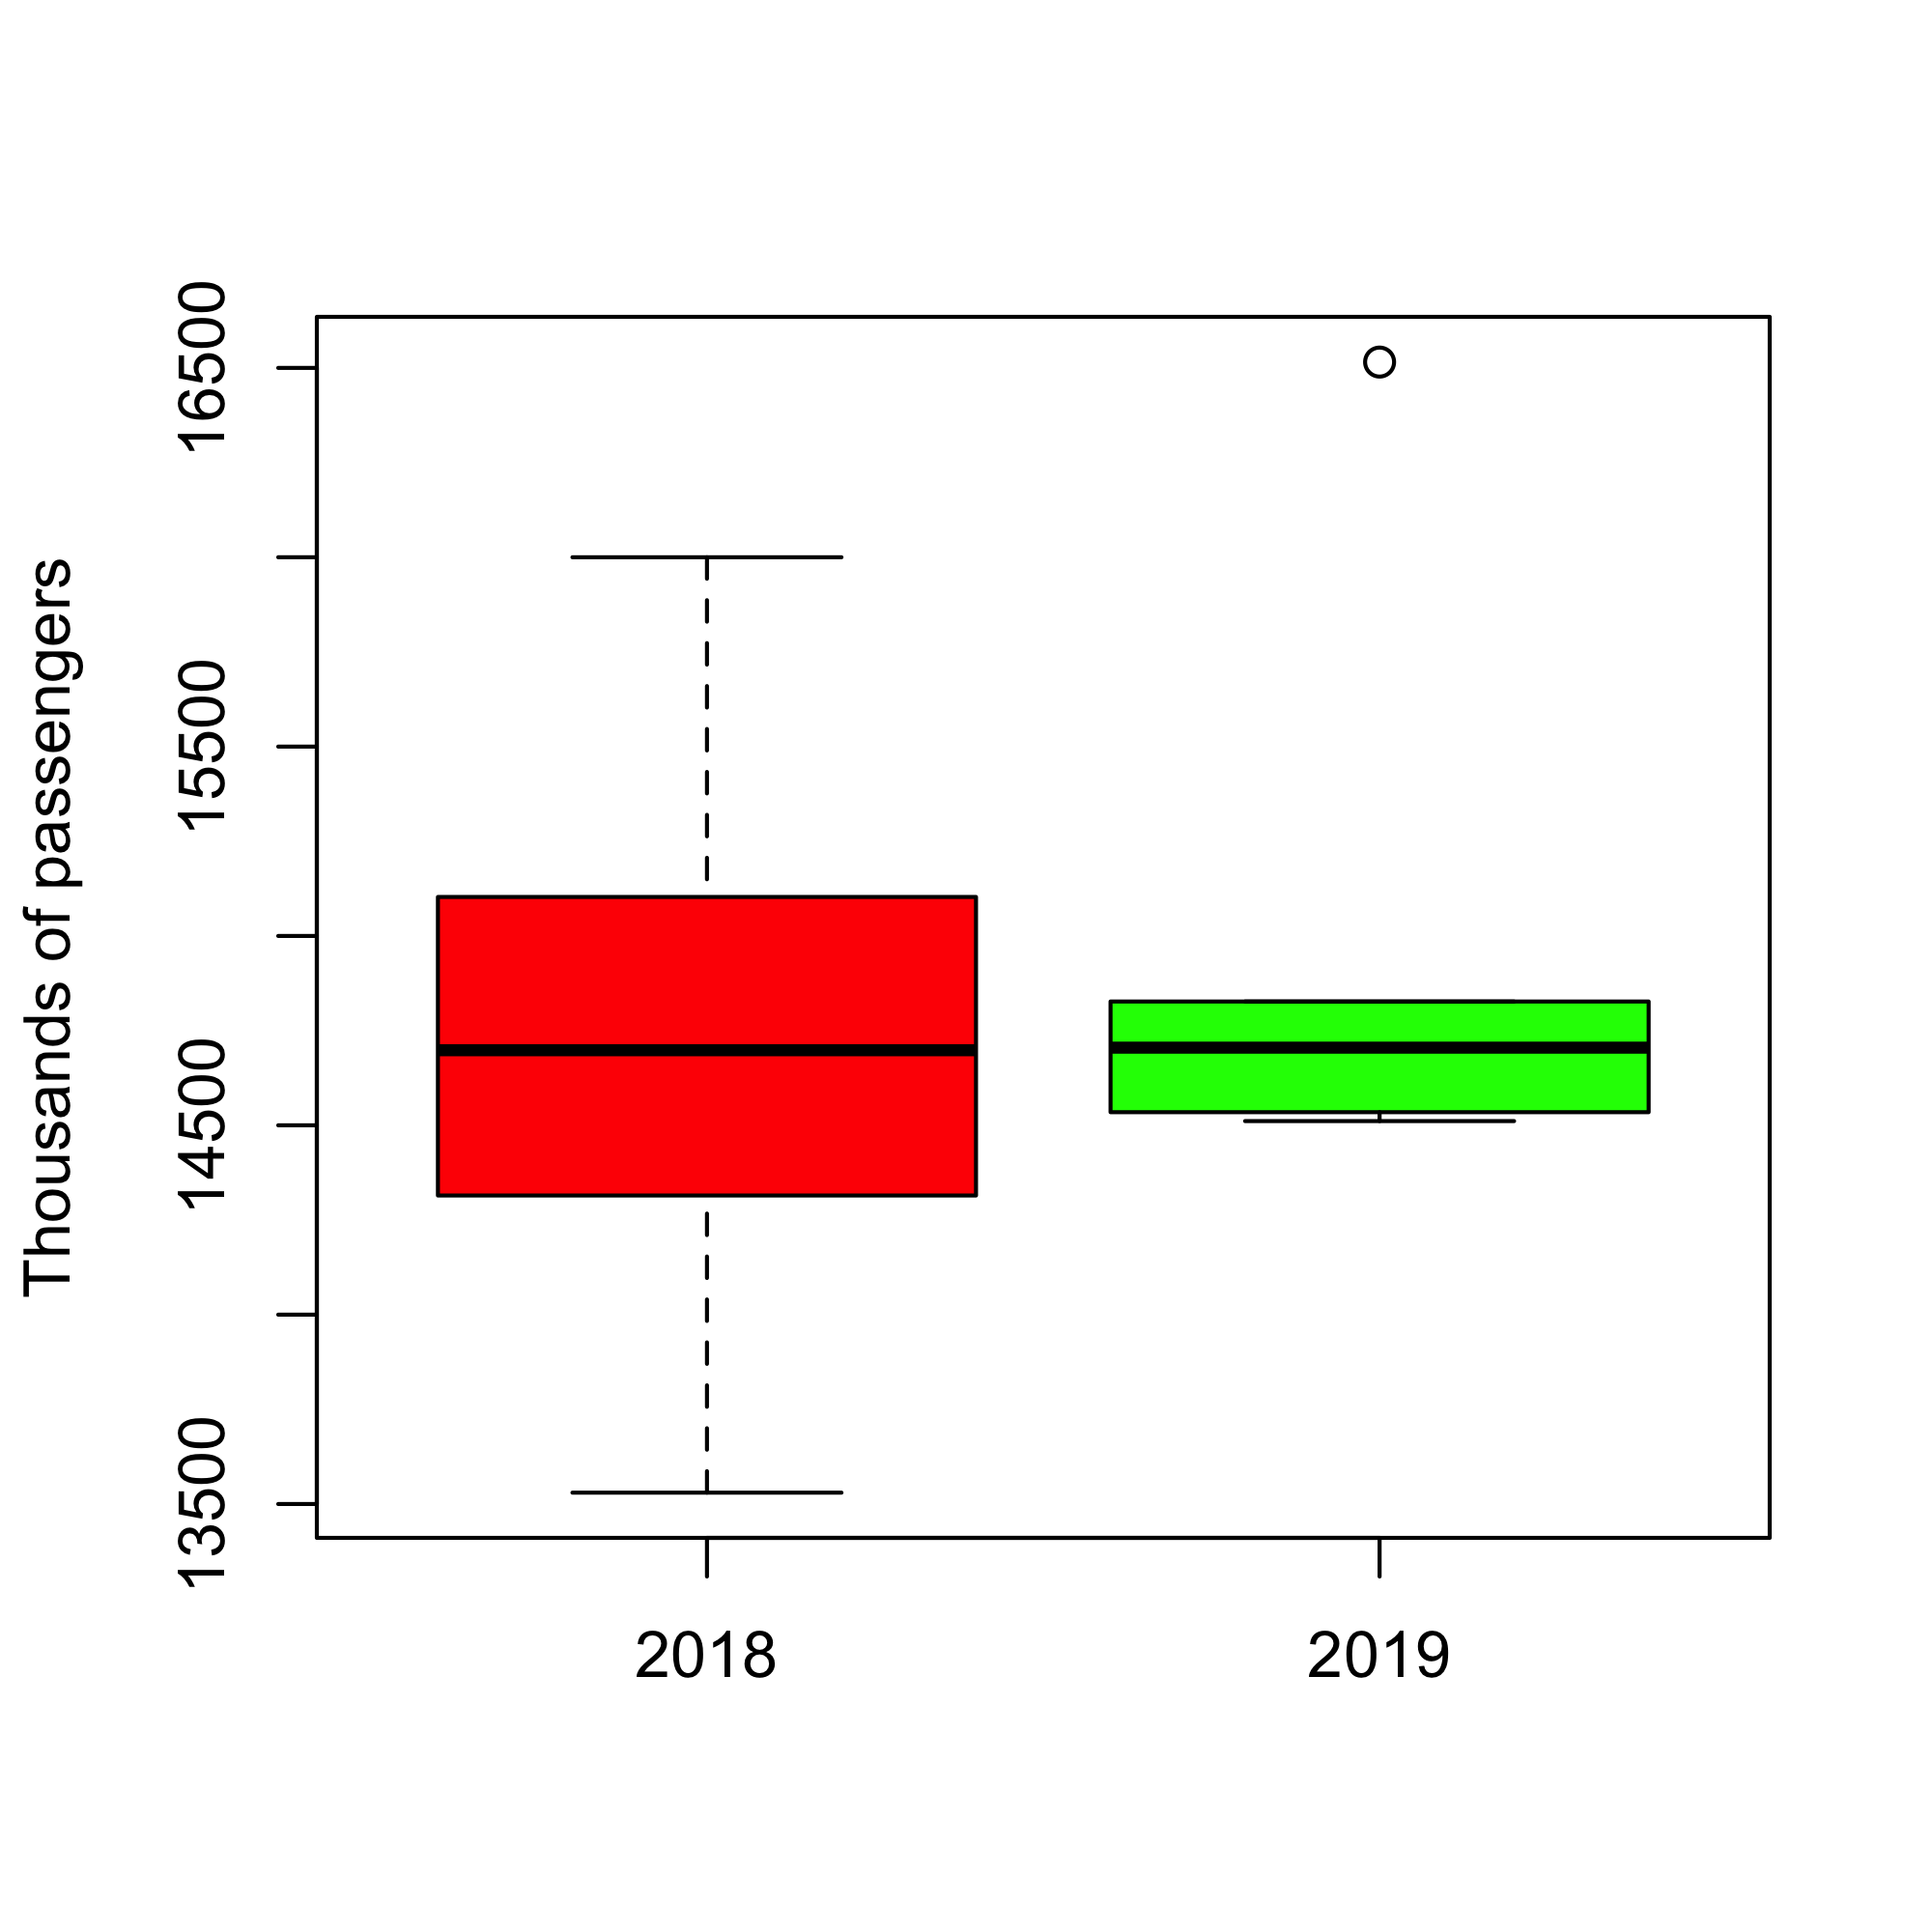
\includegraphics[width=\linewidth]{boxplot_2018_2019.png}
		\caption{}
	\end{subfigure}
	\begin{subfigure}[b]{0.3\linewidth}
		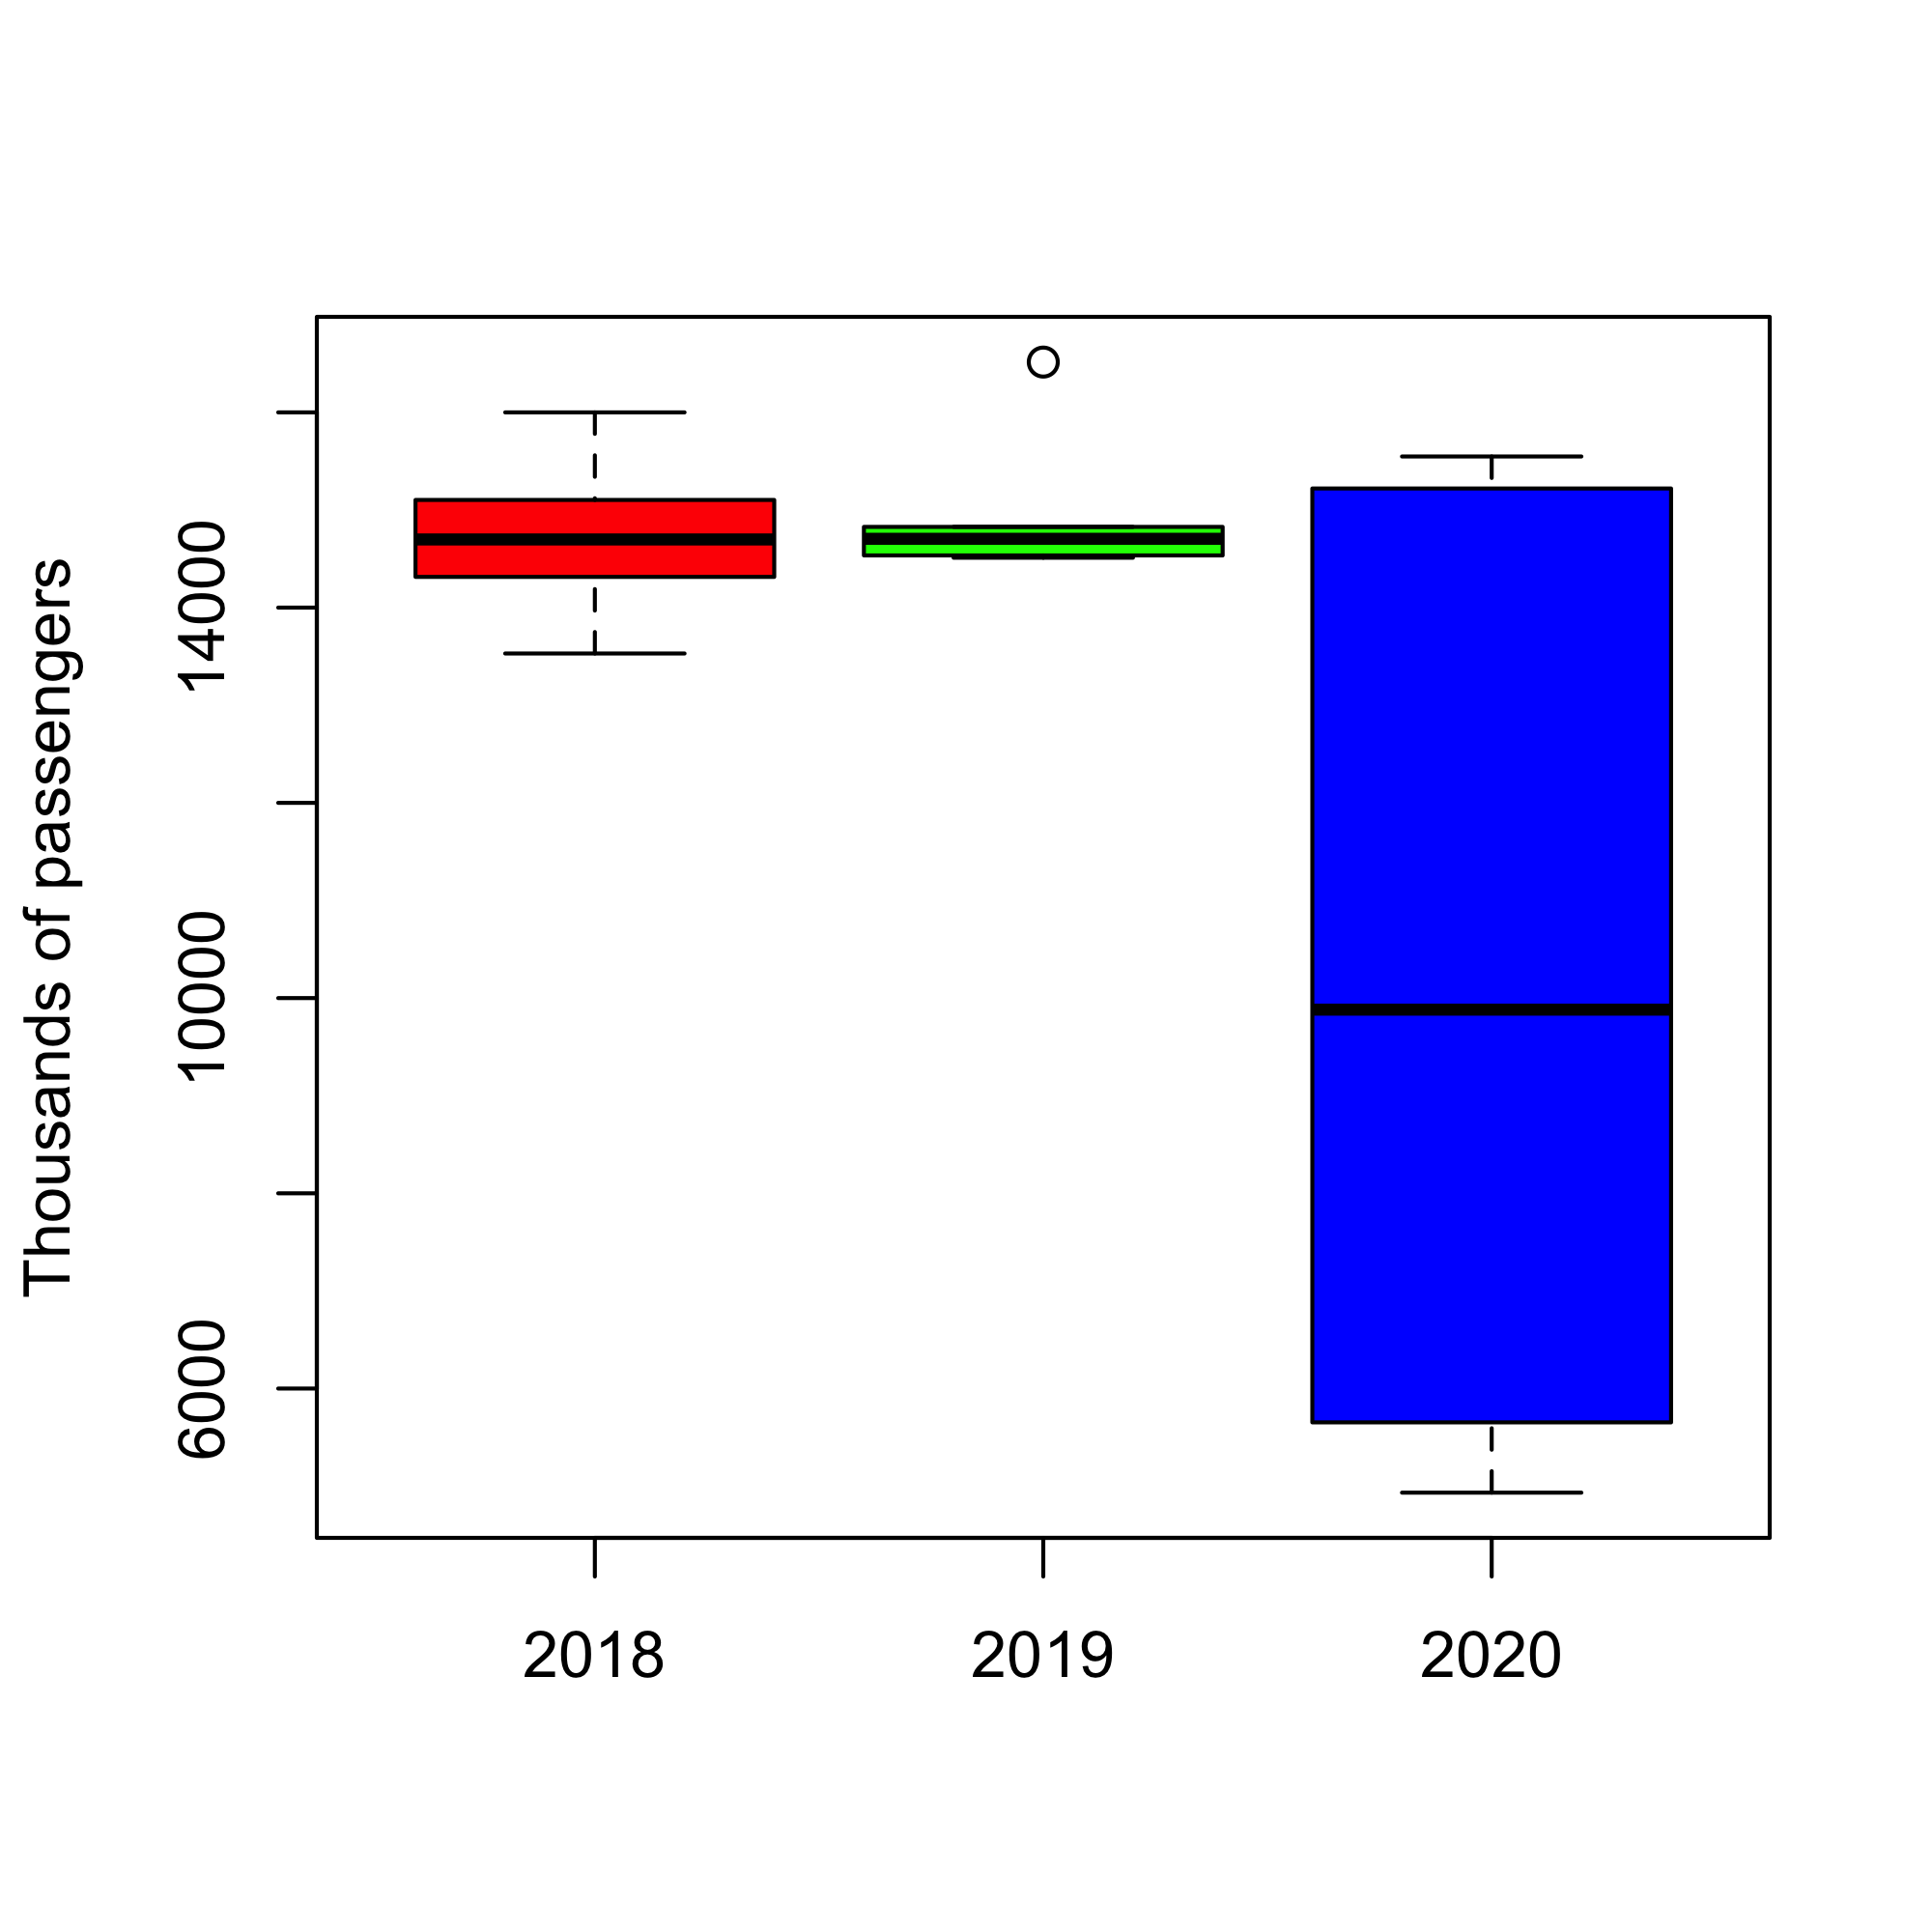
\includegraphics[width=\linewidth]{boxplot_2018_to_2020.png}
		\caption{}
	\end{subfigure}
	\begin{subfigure}[b]{0.3\linewidth}
		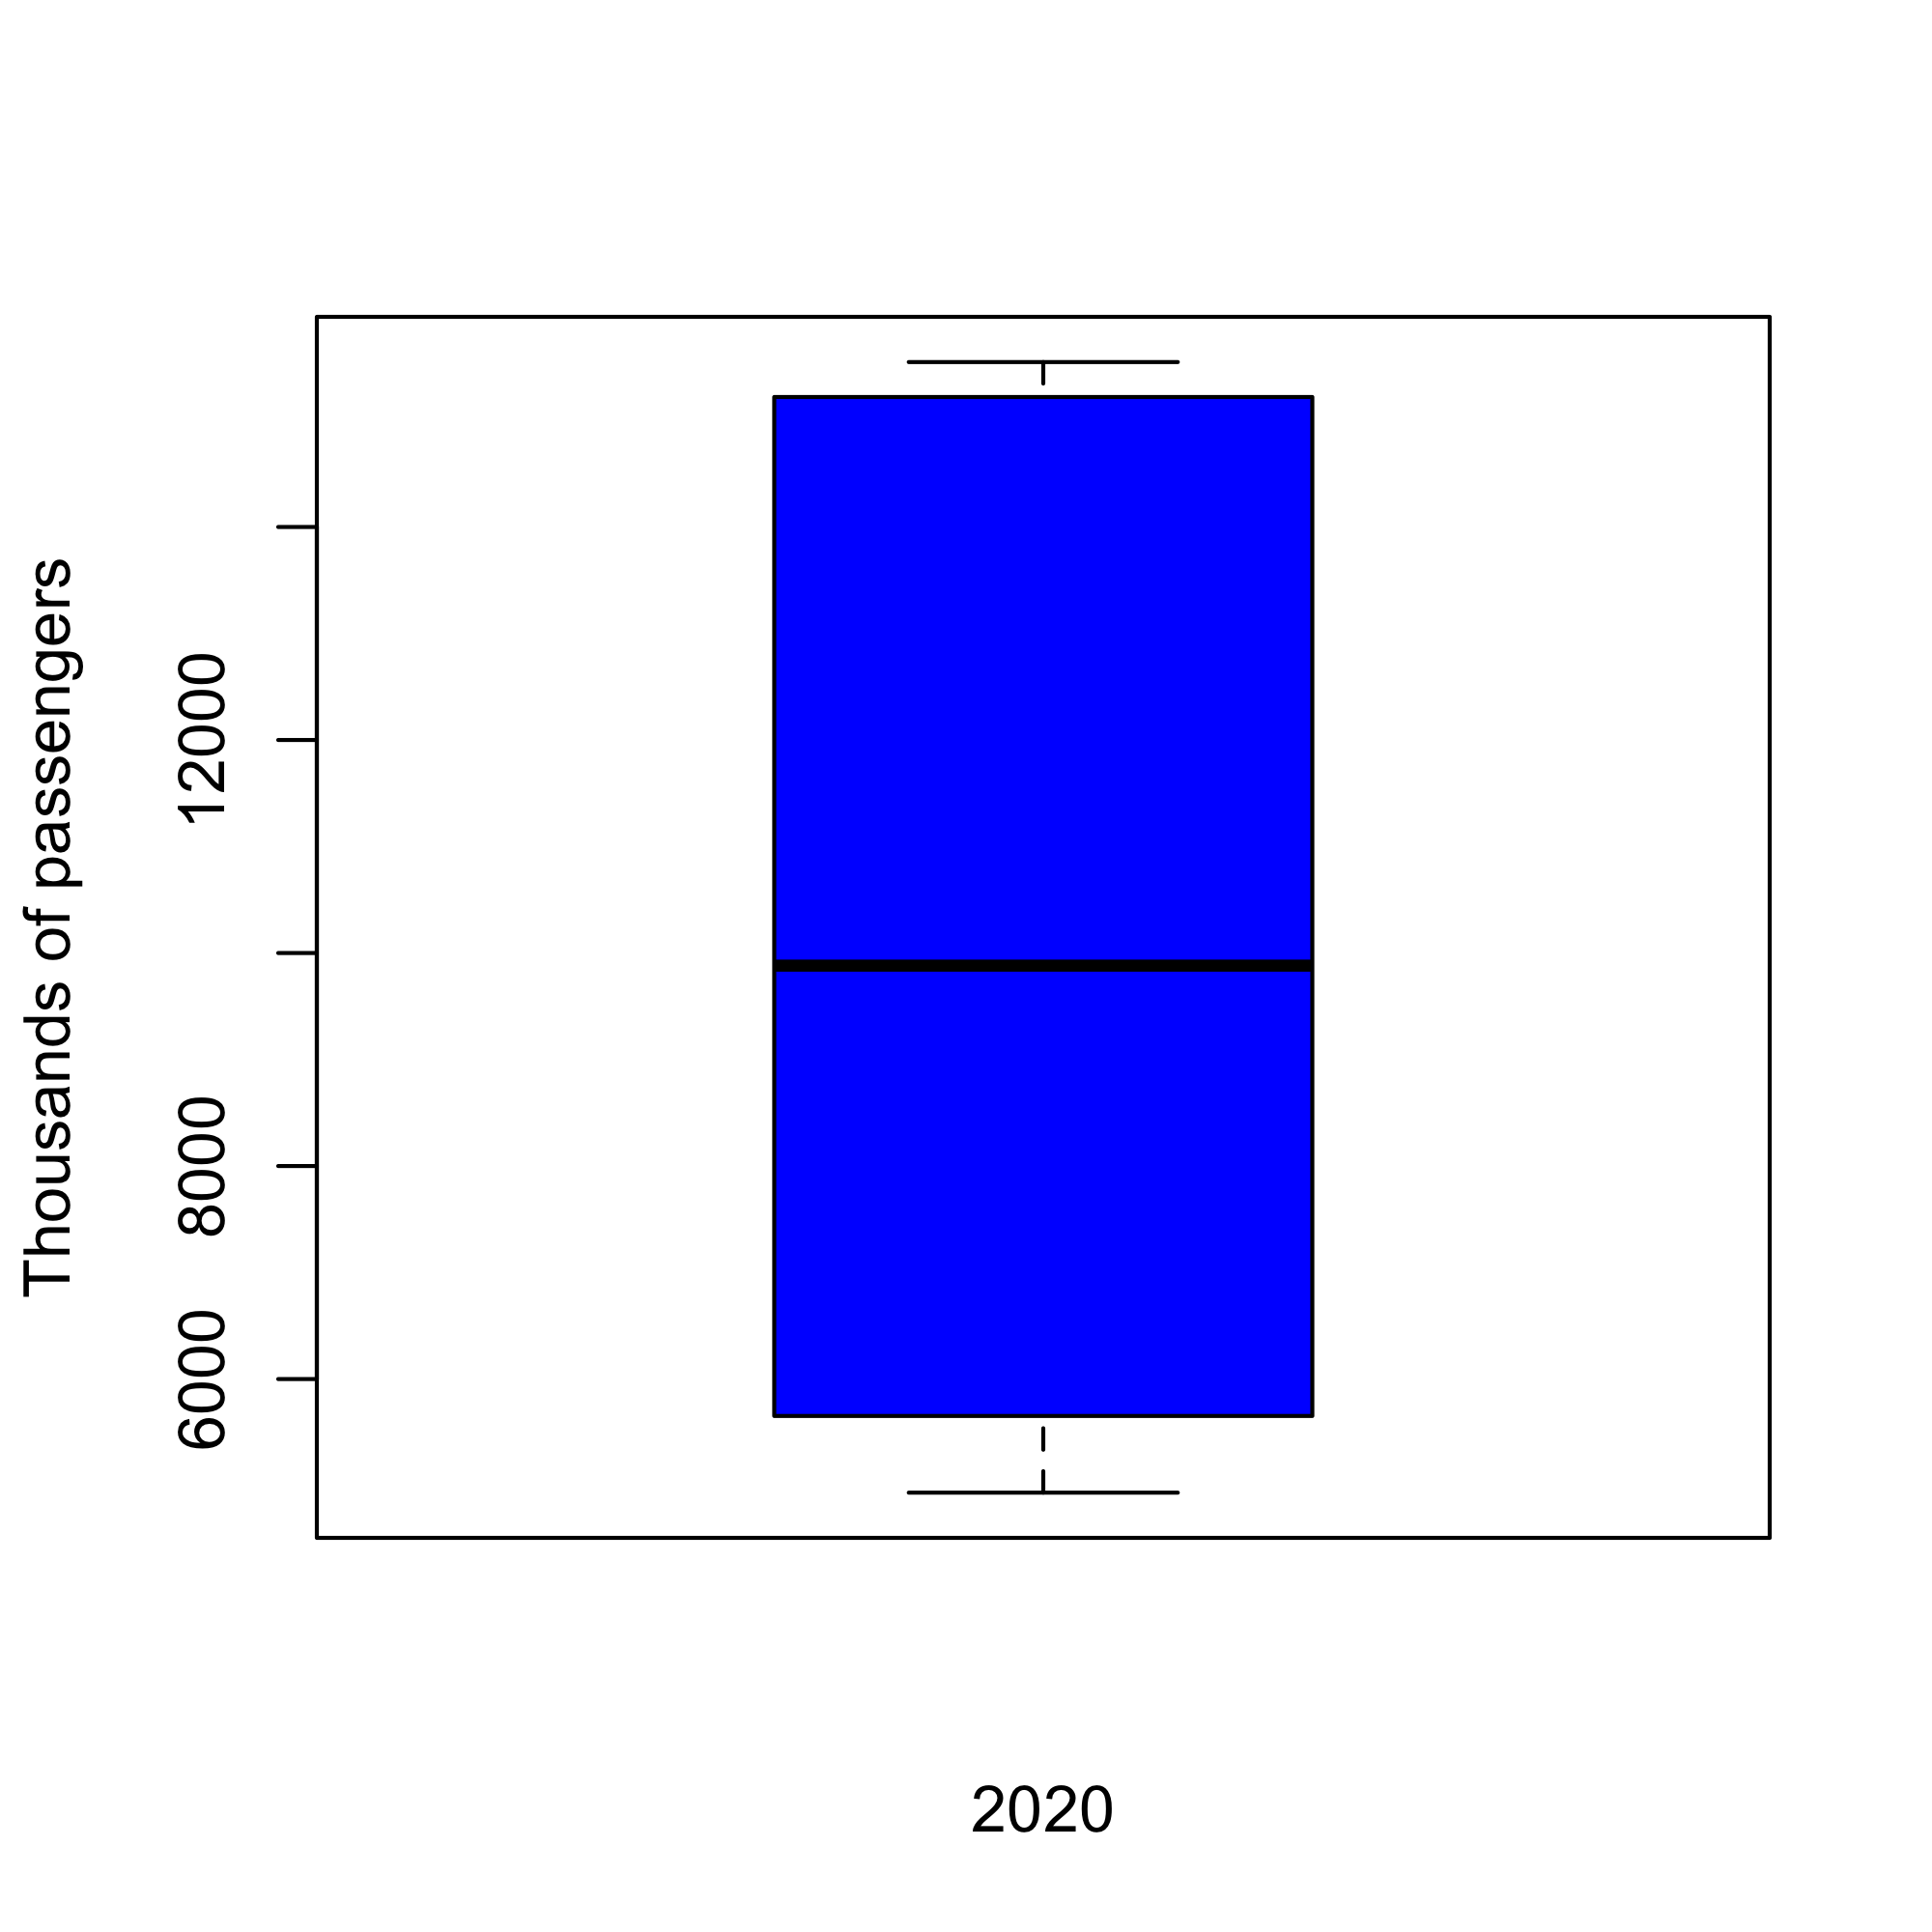
\includegraphics[width=\linewidth]{boxplot_2020.png}
		\caption{}
	\end{subfigure}
	\caption{Boxplots of January-June ridership in different years.}
	\label{fig:boxplots}
\end{figure}



\begin{figure}[h!]
	\centering
	\begin{subfigure}[b]{0.3\linewidth}
		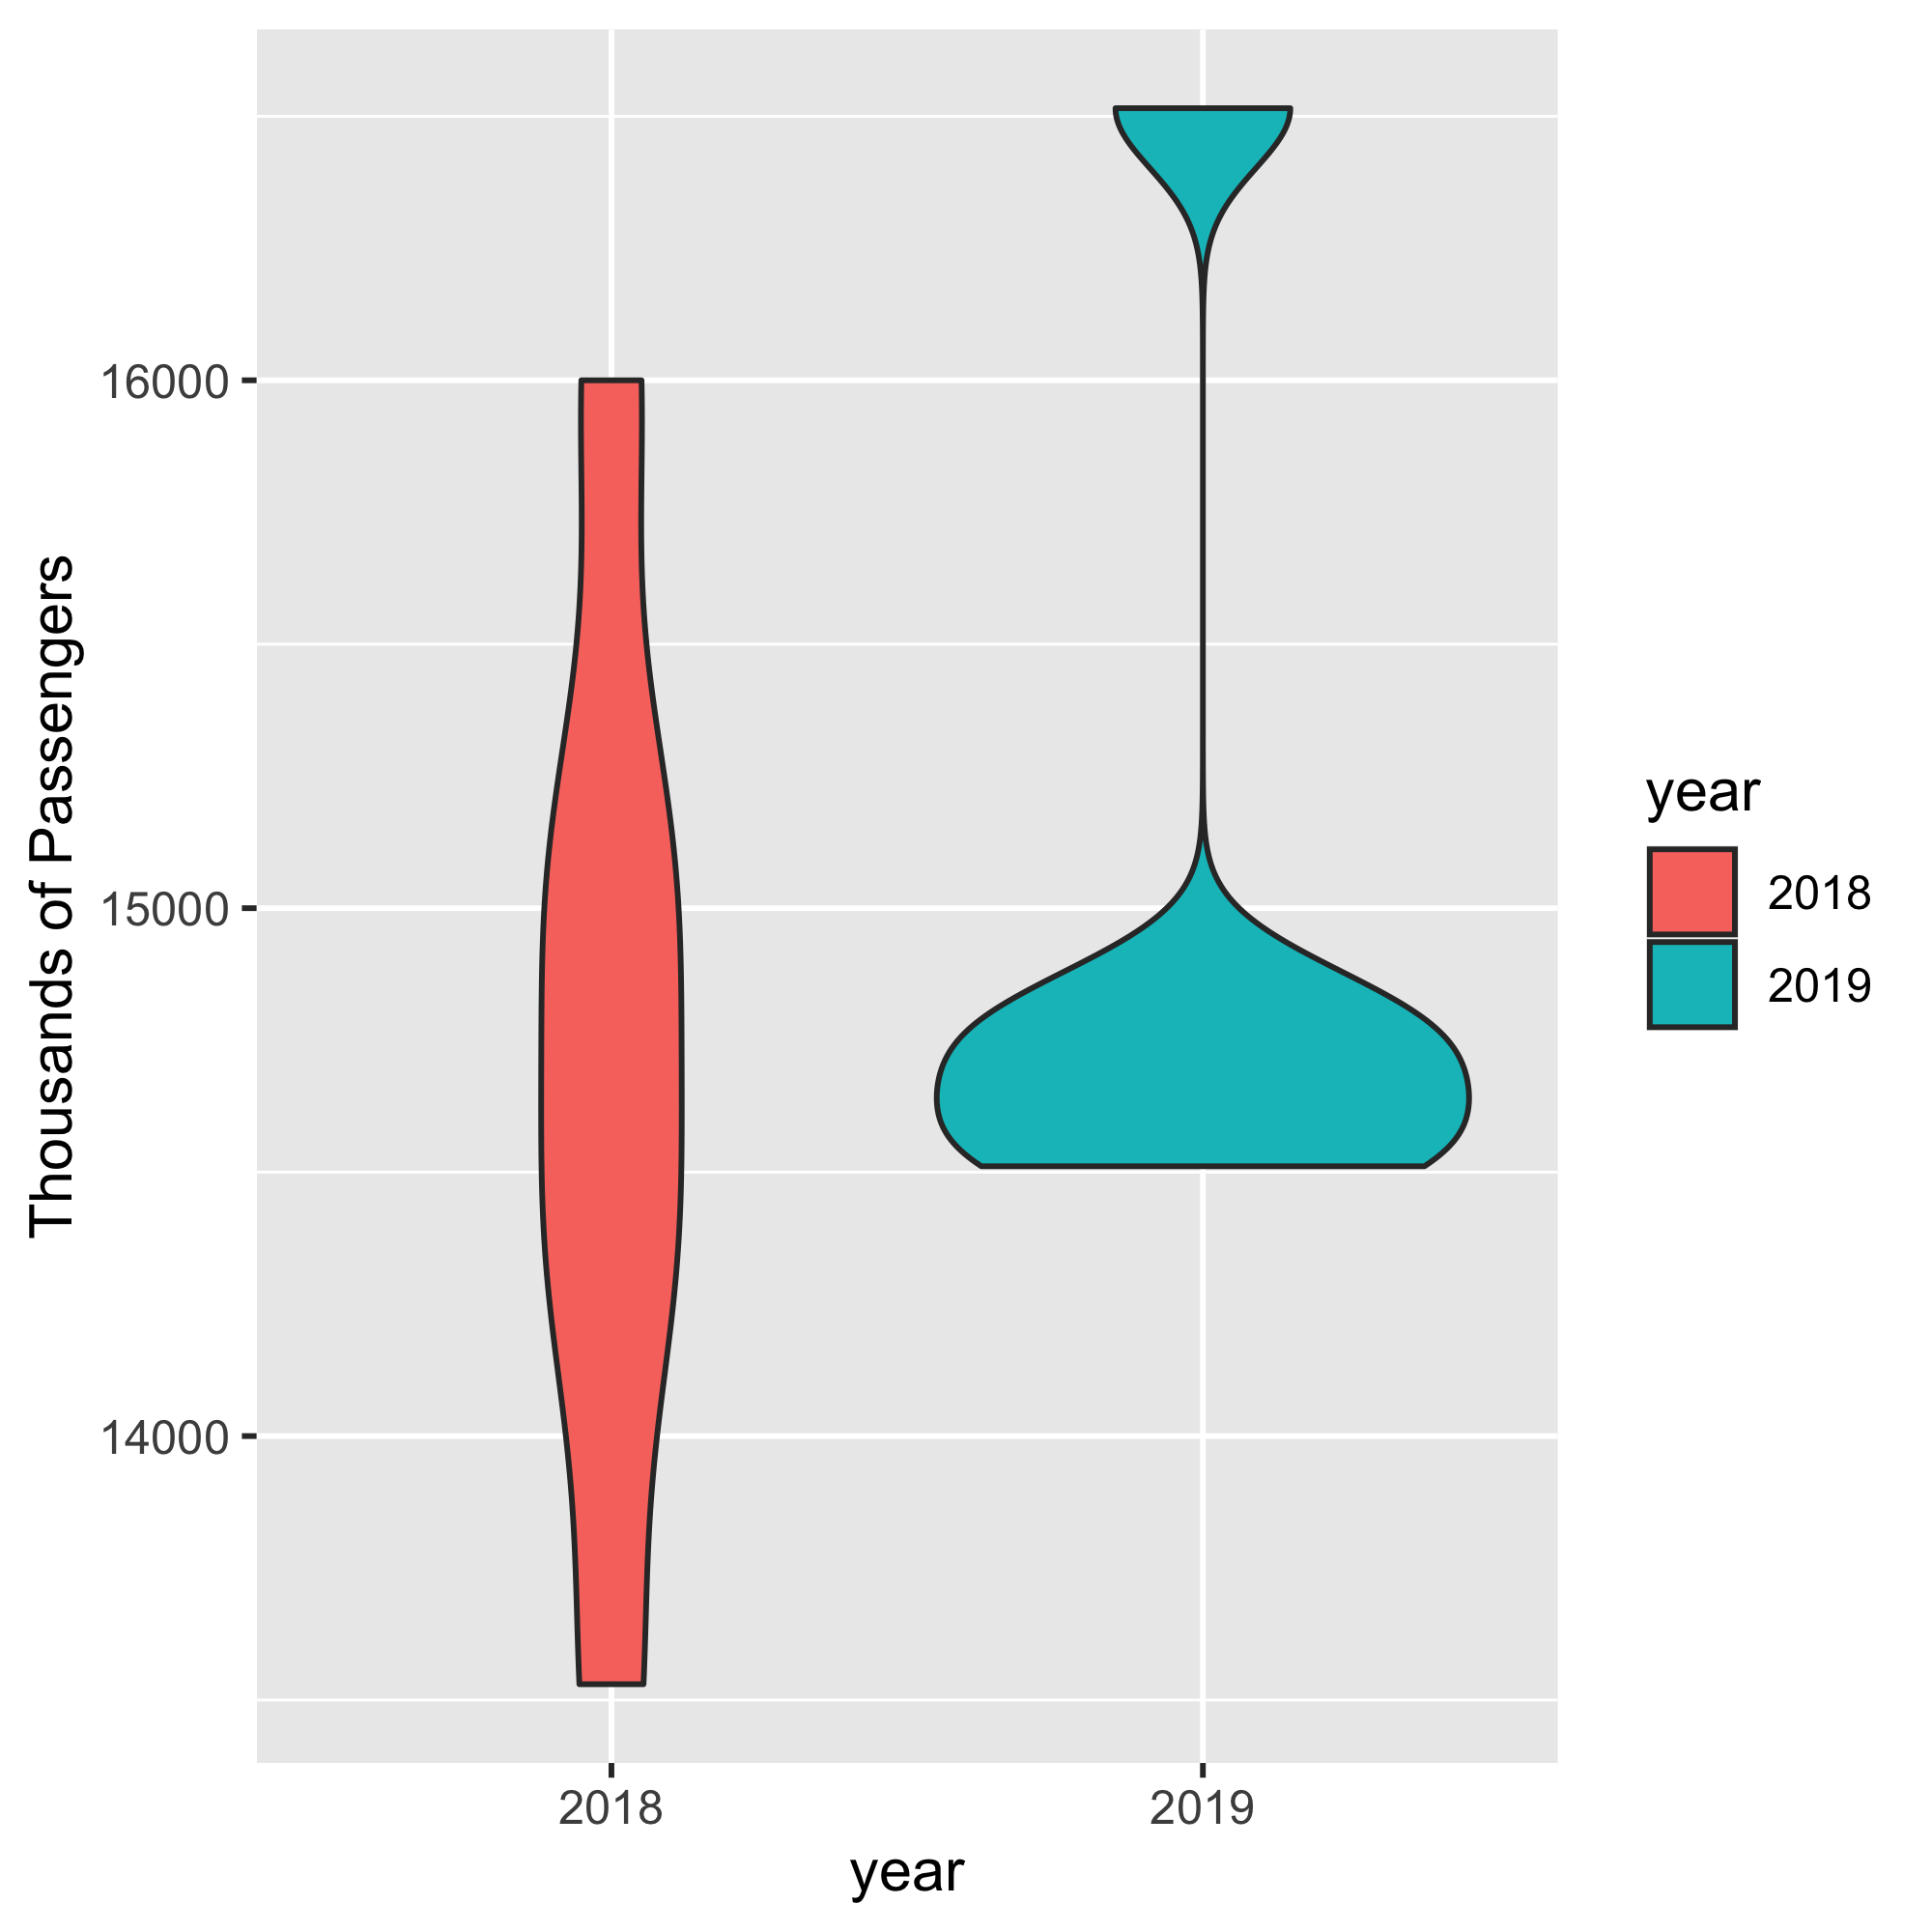
\includegraphics[width=\linewidth]{violin_plot_2018_2019.png}
		\caption{}
	\end{subfigure}
	\begin{subfigure}[b]{0.3\linewidth}
		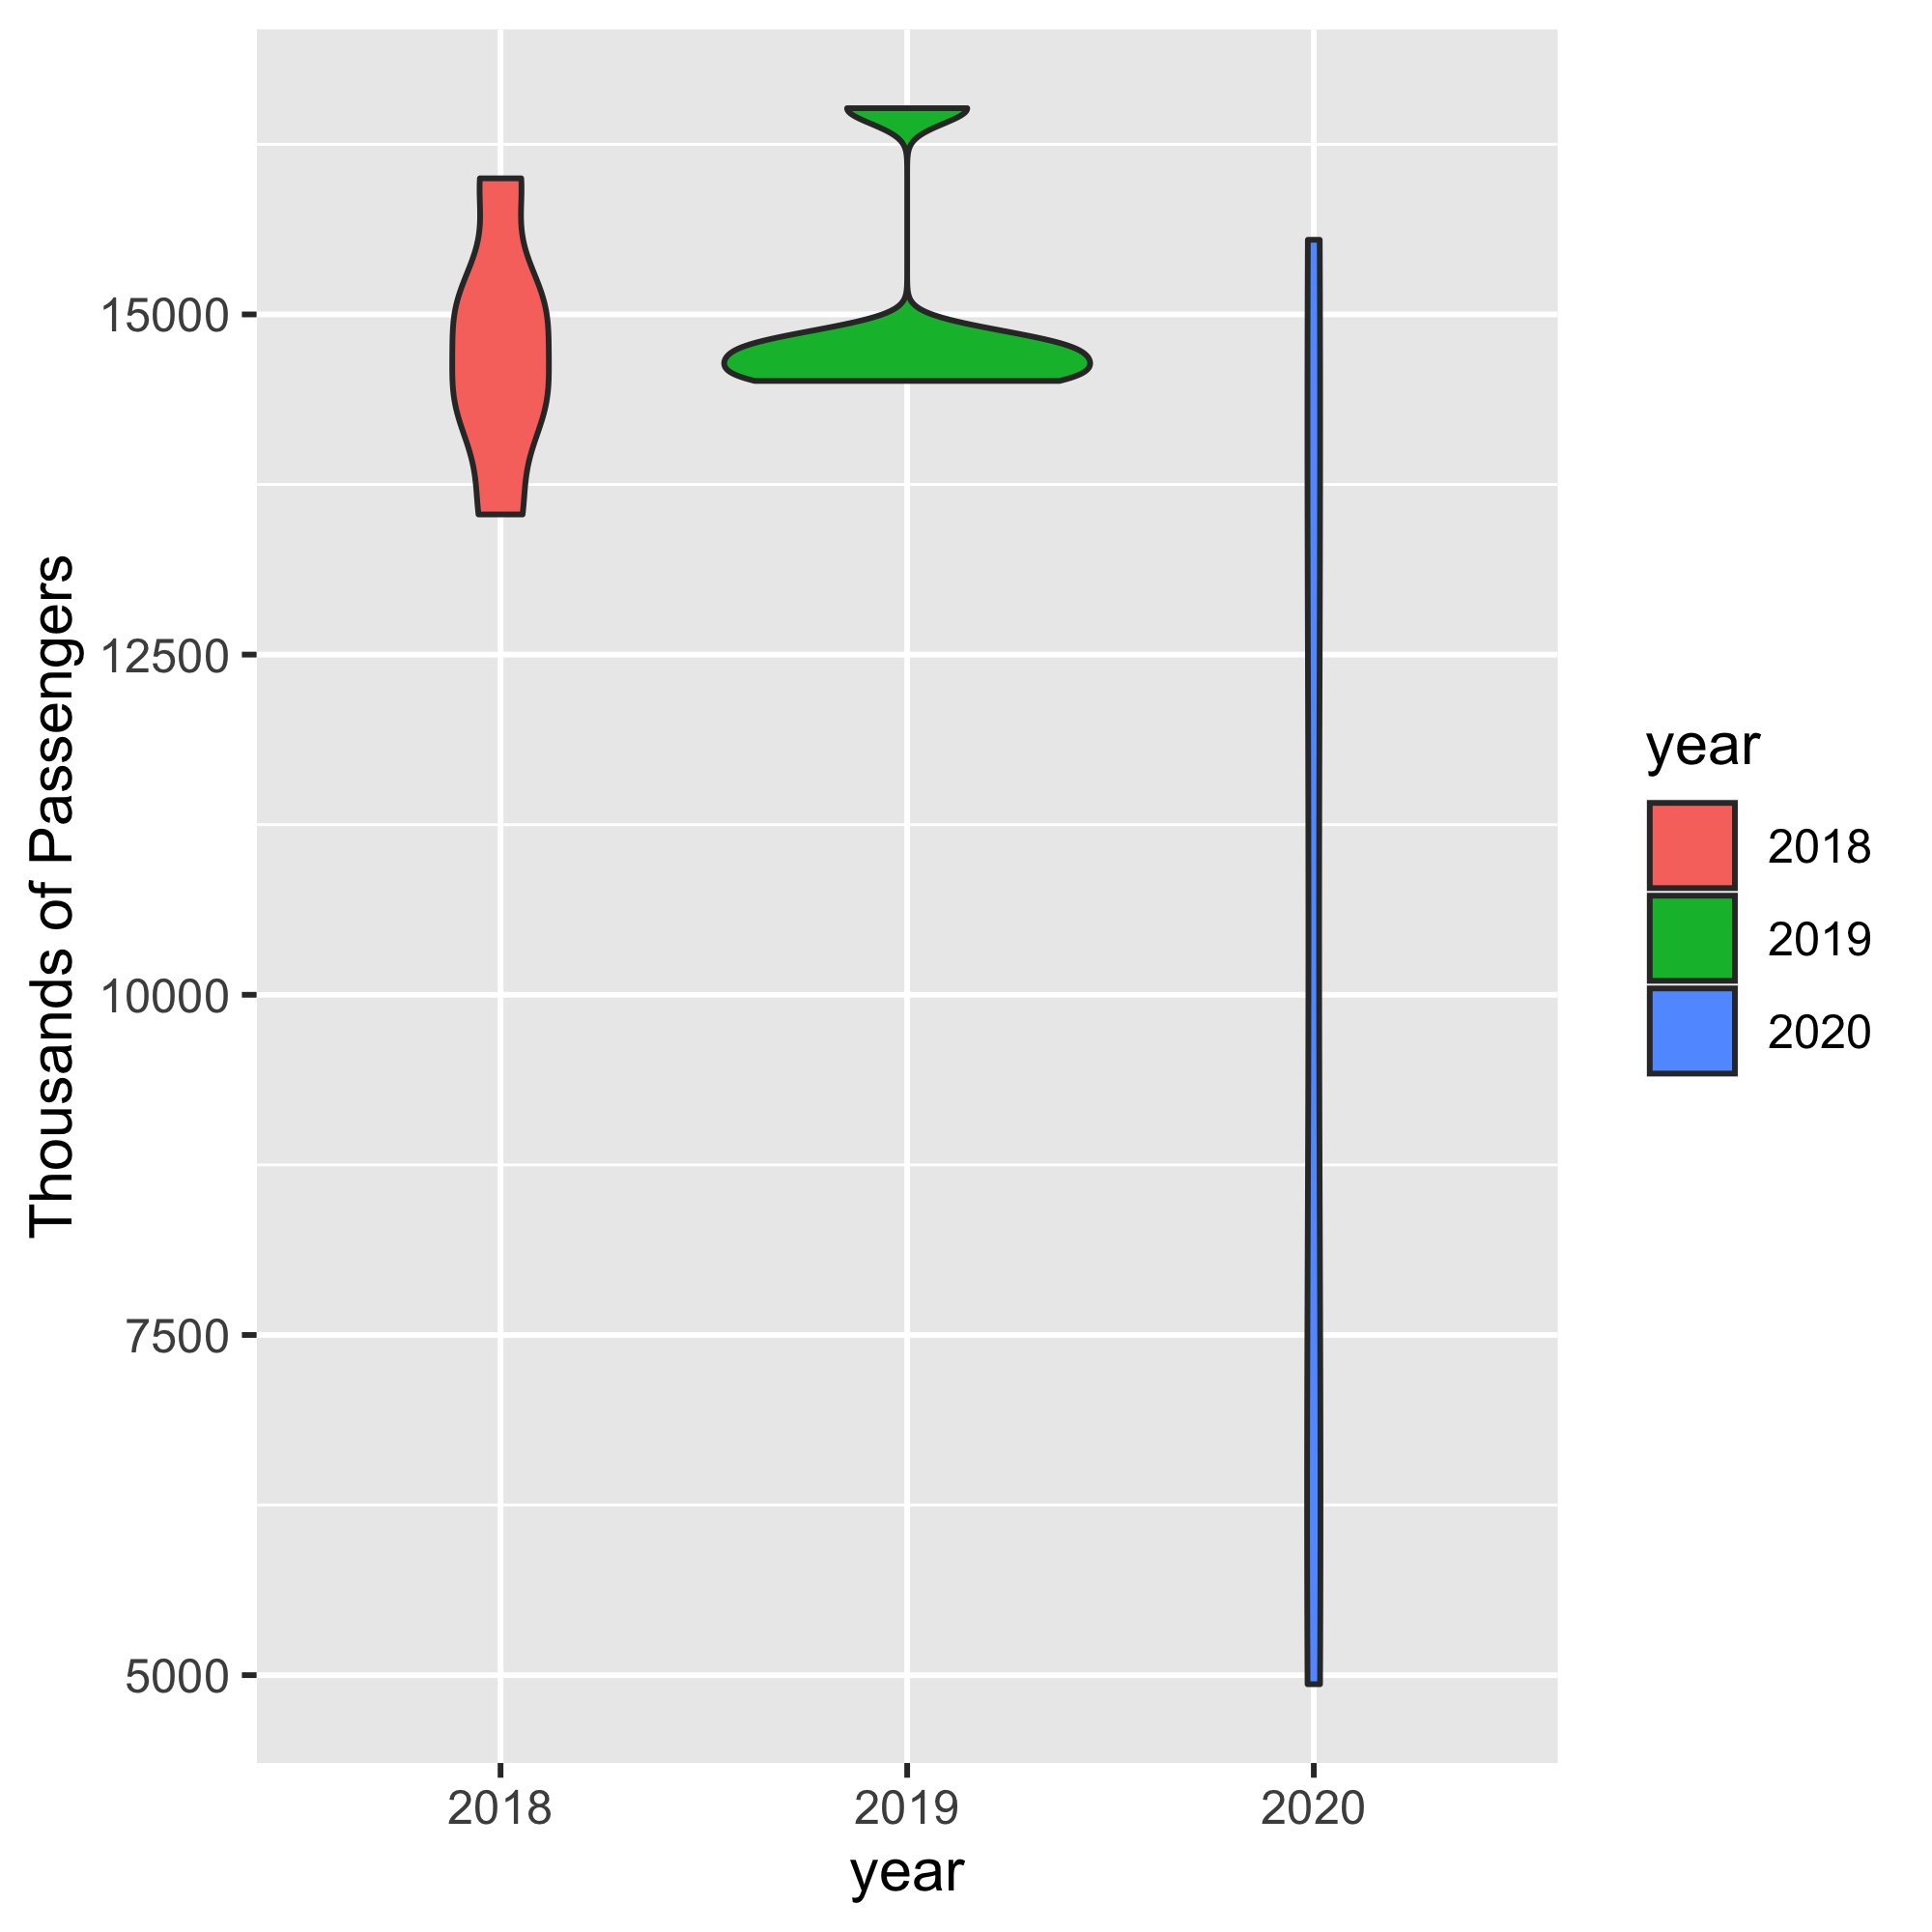
\includegraphics[width=\linewidth]{violin_plot_2018_to_2020.png}
		\caption{}
	\end{subfigure}
	\begin{subfigure}[b]{0.3\linewidth}
		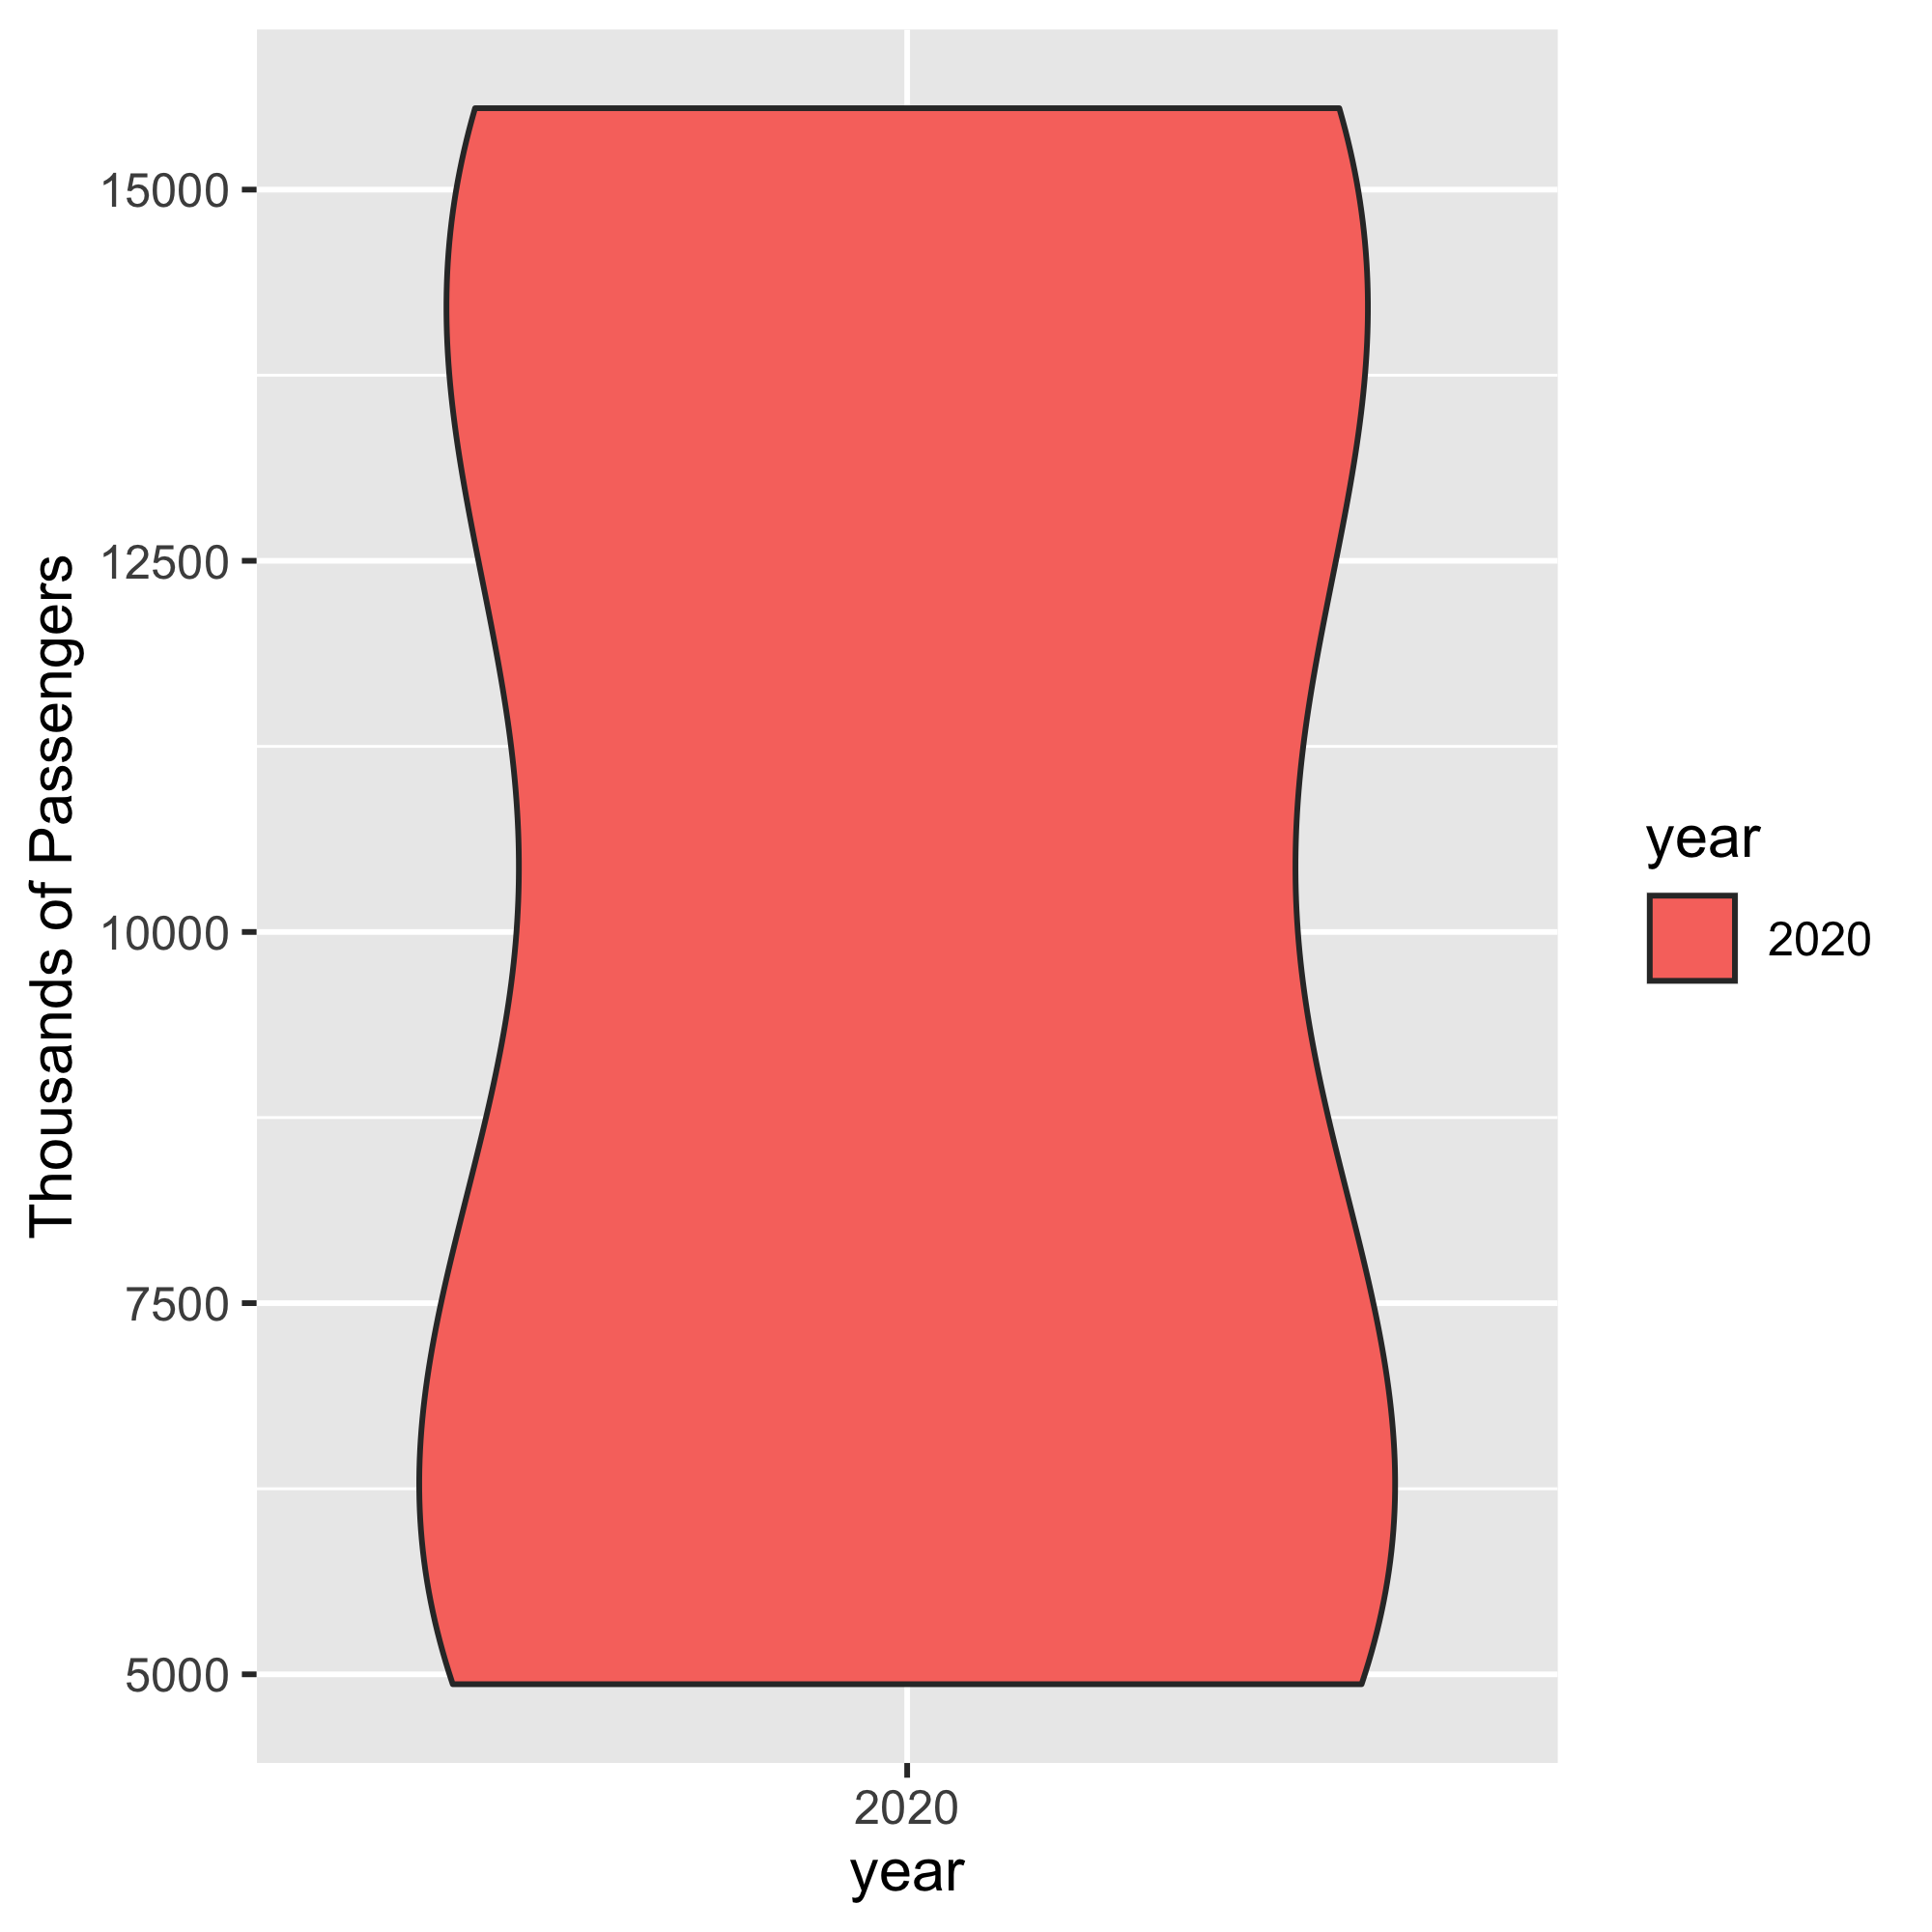
\includegraphics[width=\linewidth]{violin_plot_2020.png}
		\caption{}
	\end{subfigure}
	\caption{Violin plots of January-June ridership in different years.}
	\label{fig:violinplots}
\end{figure}

\begin{figure}[th!]
	\centering
	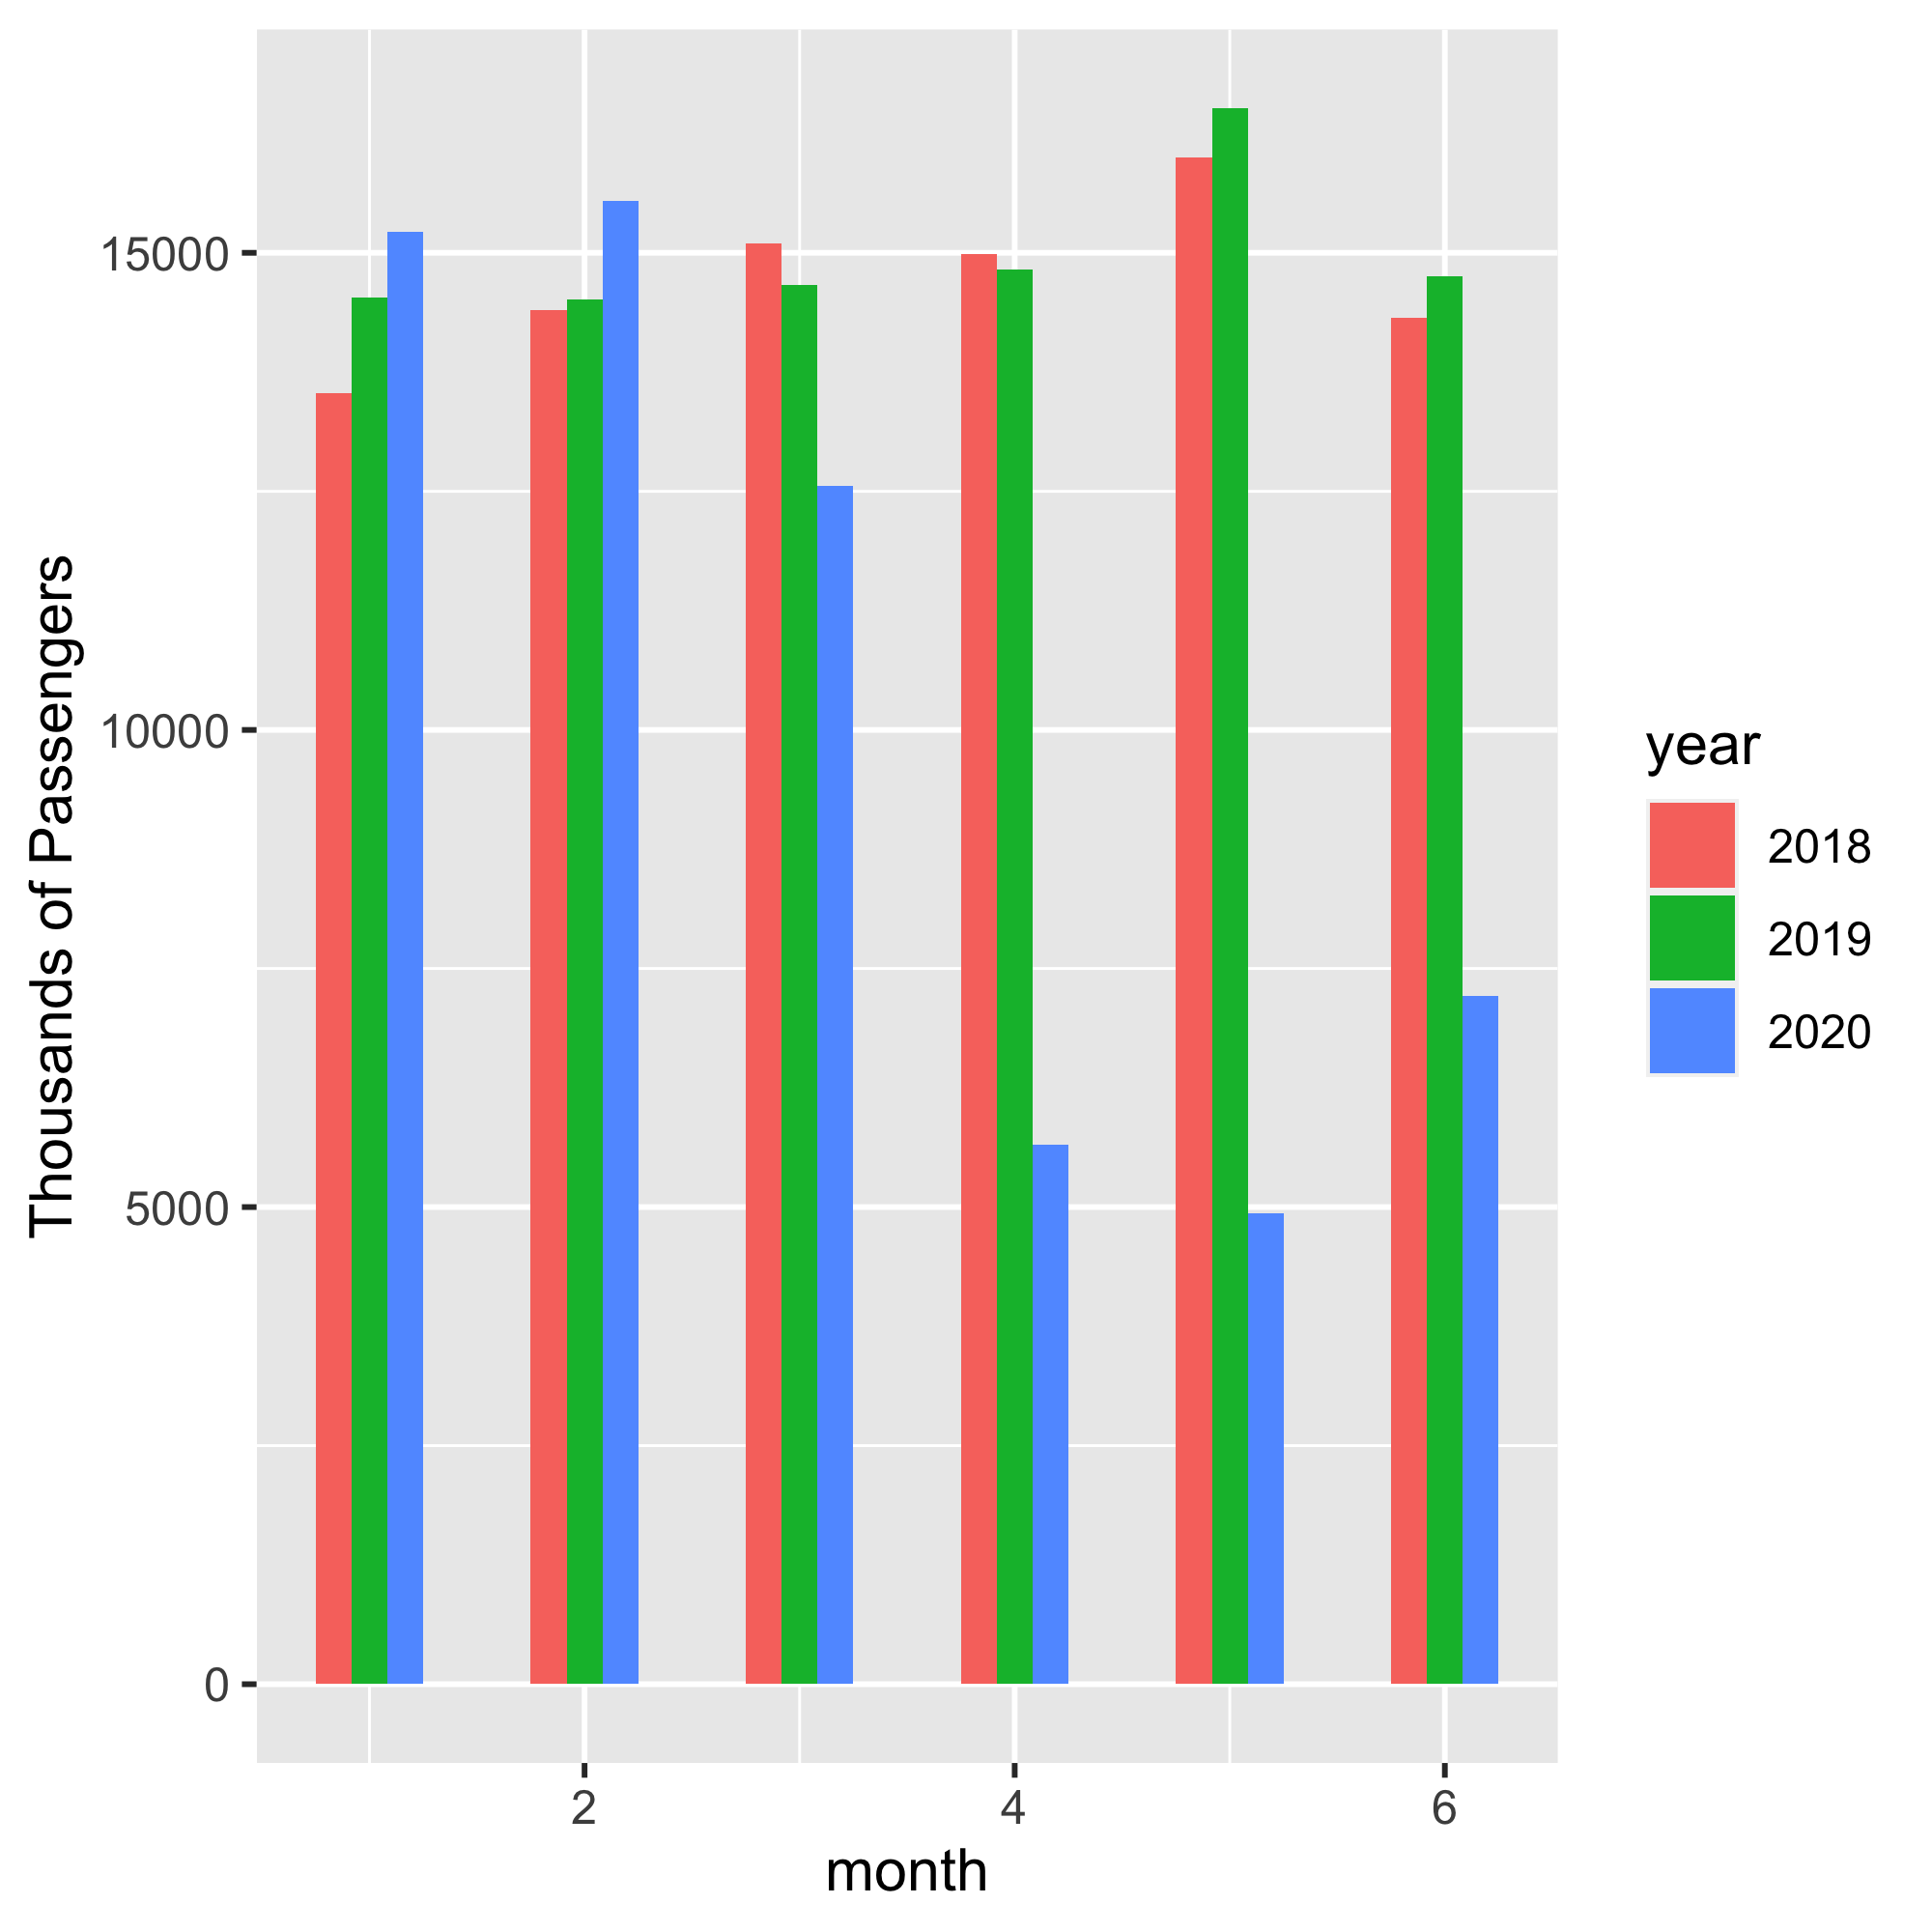
\includegraphics[scale=.1]{bar_plot_2018_to_2020}
	\caption{Bar plot of the data analysed.}
	\label{fig:barplot2018_to_2020}
\end{figure}

\section*{Conclusion}
We observe that government measures to reduce mobility in Monterrey Metropolitan area had a noticeable impact, at least with respect to Metrorrey's passengers ridership. For instance, close to 5 million people rode Metrorrey on May 2020, an 11.5 million decrease when compared to May 2019. Further analysis is needed to establish if this reduction in mobility was similar in other ways of public transport. It can also be of interest to study whether this reduced mobility stopped the spread of covid-19 in a significant way. 

%%%%%%%%%%%%%%%%%%%%%%%%%%%%

\bibliographystyle{plain}
\bibliography{refr}


%%%%%%%%%%%%%%%%%%%%%%%%%%%%
\end{document}
